\section{Halo Profiles} 
\label{sec:profiles}

The standard CDM model predicts that dark matter halos should be cuspy, asymptoting to high central densities.
This results from the inability of collisionless dark matter to redistribute kinetic energy, and is born out in numerical simulations which give rise to a family of cuspy halo profiles \citep[\eg, the NFW profile,][]{Navarro:1996gj}.
If dark matter is able to interact through scattering or the exchange of some light mediator (see \secref{sidm}), then the density of halos could instead flatten out to produce dark matter ``cores'' \citep{Spergel:1999mh}.
These interactions can also lead to an isotropization of dark matter velocity distribution, leading to more spherical halos \citep{Peter:2013}.
Thus, measurements of the radial density profiles and shapes of dark matter halos are sensitive to the microphysics governing dark matter self-interactions.
Here we explore the contributions that LSST will make towards measuring the profiles of dark matter halos in isolated small galaxies and clusters of galaxies.
We highlight these systems because they reside at opposite extremes of the galaxy mass spectrum where dark matter dominates over baryonic processes that can also alter the shapes of halos.

\subsection{Dwarf Galaxies as Lenses \Contact{Yao}}
\Contributors{Yao, Annika, James, Tony, Manoj?, ...}
\label{sec:halo_profile_group}

%\ADW{I think we need to make it clear early on that we are talking about dwarfs beyond the Local Group.}
%\ADW{I think that the structure of this section could be: (1) intro to the core-cusp problem (more focus than missing satellites), (2) description of the LSST lensing projections, (3) connect back to dark matter physics (i.e., how will a lensing signal help us solve cusp/core.}

Dwarf galaxies ($M_\star \lesssim 10^{9} \Msun$) provide the best visible tracers of low-mass dark matter halos. 
The relatively low baryonic content makes dwarf galaxies sensitive probes of  dark matter physics through the shape of their dark matter halo profiles. 
In particular, the ``core-cusp'' problem in dwarf galaxies has been cited as one of the most significant challenges to CDM \citep[\eg,][]{2010AdAst2010E...5D,Bullock:2017xww}.
The standard CDM model predicts that dark matter halos should have steeply rising (``cuspy'') central densities in contrast to the shallower (``cored'') mass profiles that are observationally inferred for many dwarf galaxies.  
Evidence for cored profiles exists for Milky Way satellite galaxies from kinematic and theoretical studies \citep[\eg][]{Walker:2009, 2012ApJ...759L..42P}, and is stronger when one studies the inner density profiles of dwarf galaxies based on high-resolution neutral hydrogen surveys \citep[\eg][]{Begum:2008,Hunter:2012,Cannon:2011,Oh:2015}. 
Many of these observations show inferred central slopes of the dark matter density profile, $\rho(r) \sim r^{\gamma}$, that are significantly shallower ($\gamma \approx 0$--$0.5$) than the CDM prediction $\gamma \approx 0.8$--1.4 \citep{Navarro:2010}.

A wide range of solutions to the core-cusp problem have been proposed including observational, astrophysical, and dark matter explanations.
From a dark matter perspective, SIDM can significantly suppress the the central density of halos.
A self-interaction cross-section of $\sigma / m_\chi \sim 1 \cmg$ can explain the diversity of rotation curves seen in low-mass spiral galaxies \citep[\eg][]{1504.01437,2017PhRvL.119k1102K,Tulin:2017ara}.
In addition, ultra-light or fuzzy dark matter has also been suggested as a possible solution to the core-cusp problem through the formation of uniform density solitonic cores \citep[\eg][]{1502.03456,Hui:2017}. 
However, baryonic feedback remains a major complication for interpreting central density profile measurements in a dark matter context \citep{1996MNRAS.283L..72N,2005MNRAS.356..107R,2008Sci...319..174M,2012MNRAS.421.3464P,Madau:2014,Read:2016}. 
If dwarf galaxies form enough stars, energy from SN explosions can flatten the profiles of dark matter and baryons; however, if too many stars are formed, the excess baryonic mass can have the opposite effect of steepening the slope of the central density profile \citep{Bullock:2017}.
Technical challenges in implementing multi-phase gas and baryonic physics make it difficult to directly address and calibrate baryonic predictions based on hydrodynamical simulations \citep{Tollet:2016,1611.02281,Sawala:2016}.
However, one key prediction is that the creation of cores will be sensitive to the exact star formation history \citep[\eg][]{governato2012,dicintio2014,onorbe2015,Read:2016,read2018,1811.11768,2019MNRAS.tmp....3R}.
Thus, robust measurements of both the stellar and dark matter mass of dwarf galaxies is essential to investigate the effect of baryonic feedback on the central dark matter density.
In addition, it has been argued that significant observational and astrophysical systematics, such as beam smearing, center offsets, inclinations, and non-circular motions can bias central density measurements toward flatter profiles \citep[\eg][]{astro-ph/0006048,2004ApJ...617.1059R,2008AJ....136.2761O,2016MNRAS.462.3628R}. 
Thus, accurate independent measurements of dwarf galaxy density profiles are critical.

LSST can provide joint statistical measurements of both the central density and stellar content of dwarf galaxies. 
The stacked gravitational weak lensing signal from a large sample of dwarf galaxies will provide the most direct measurement of the amount and distribution of dark matter.  
In this section we predict LSST's sensitivity to a stacked weak lensing signal from dwarf galaxies.

\paragraph{Dwarf galaxy lenses:}
We are interested in estimating the number of isolated dwarf galaxies accessible to LSST as a function of dark matter halo mass.
To predict the abundance of the dwarf  galaxy sample, we assume the mass-to-light ratio derived from the subhalo abundance matching and the global galaxy luminosity function \citep{2015MNRAS.451.1540L}.
We use this predicted galaxy luminosity to estimate the limiting redshift for dwarf galaxy detection as a function of galaxy halo mass for two LSST limiting magnitudes: $r \sim 25$ and $r \sim 27$. 
\figref{dwarf_redshift} shows that to probe dark matter halos with mass $\lesssim 10^9 \Msun$, it will be necessary to select galaxies at $z < 0.01$. 
While selecting very low-$z$ galaxies with photometric data is challenging, current projects like the SAGA Survey \citep{Geha:2017} have shown that it is possible using data from SDSS. 
Future large, multi-object spectrographs (\eg DESI) will greatly expand the spectroscopic data for training these selections. 
It will also be possible to use morphological information to select nearby dwarf galaxies.
LSST will be able to distinguish a dwarf galaxy with $M_V=-14$ from background galaxies of the same apparent magnitude out to a distance of $\roughly 100 \Mpc$ \citep[Section 9 of][]{0912.0201}.

\begin{figure}
\centering
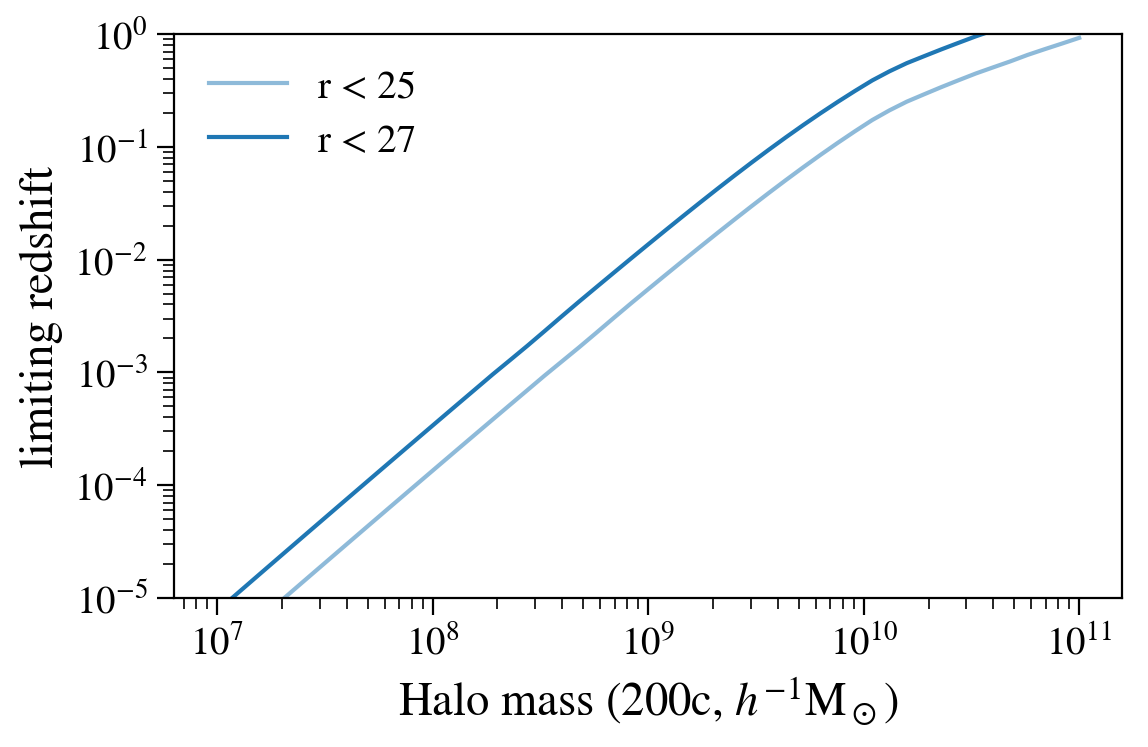
\includegraphics[width=0.7\columnwidth]{halo_mass_redshift_log}
\caption{\label{fig:dwarf_redshift} Limiting redshift for detecting a dwarf galaxy that lives in a dark matter halo of certain masses, assuming a luminosity--halo mass relation from abundance matching.}
\end{figure}


\paragraph{Source galaxies:}
The conservative LSST 10-year ``gold'' sample for cosmic shear measurements of dark energy is expected to have a source galaxy density of $\roughly 27 \amin^{-2}$ \citep{Chang:2013,1809.01669}. 
However, we expect that the dwarf lensing analysis can retain significantly more source galaxies for the following reasons.
(1) Our measurement uncertainty is dominated by the low number of dwarf galaxy lenses, rather than the  multiplicative shear measurement bias that must be strictly controlled for dark energy measurements. This allows us to include fainter, smaller, and more blended sources.
(2) Unlike the lenses used for cosmic shear measurements, the dwarf galaxy lenses are at very low redshift. This means that most detected sources are background galaxies.
(3) We expect to be able to combine shape measurements from multiple filters, which could increase the source density by $\roughly 80\%$. 
Combining these factors, we estimate a source galaxy density of $50 \amin^2$, which is consistent with the fiducial, multi-band estimate of \citet{Chang:2013}.
The primary focus of the source galaxy selection will be to avoid catastrophic \photoz outliers (low-$z$ galaxies reported at high-$z$), which are typically less than a few percent in current surveys \citep{1406.4407}. 
%\Photoz algorithms incorporating machine learning currently achieve better performance, giving posterior p(z) estimating which enables cuts on suspect source galaxies. 

\paragraph{Sensitivity:}
We calculate the expected strength of a lensing signal for three different bins in halo mass,  $M = \{10^{10} \Msun, 3\times10^9 \Msun, 10^{9} \Msun \}$, each with a width of $0.5$\,dex in mass. 
These samples corresponds to $N = \{1.2\times10^8, 7.8\times10^6, 1.6\times10^5\}$ dwarf galaxies out to a redshift of $z = \{0.35, 0.07, 0.014\}$, respectively.
Source galaxies are placed at $z = 1.2$ with a density of $50 \hbox{ arcmin}^{-2}$ and a shear uncertainty of $\sigma_\gamma = 0.25$.
We model the mass distribution in each dwarf galaxy with an NFW halo assuming the concentration-mass relationship from \citet{1809.07326}.
We calculate the shear from the stacked dwarf galaxy lens sample using \code{colossus} \citep{2018ApJS..239...35D}, assuming that each lens is placed at the limiting detectable redshift.
The results are shown in \figref{dwarf_sn}, where we find that LSST has the potential to measure the lensing shear with ${\rm S/N} \gtrsim 10$ for halos with $M \gtrsim 3 \times 10^9$.

\begin{figure}
\centering
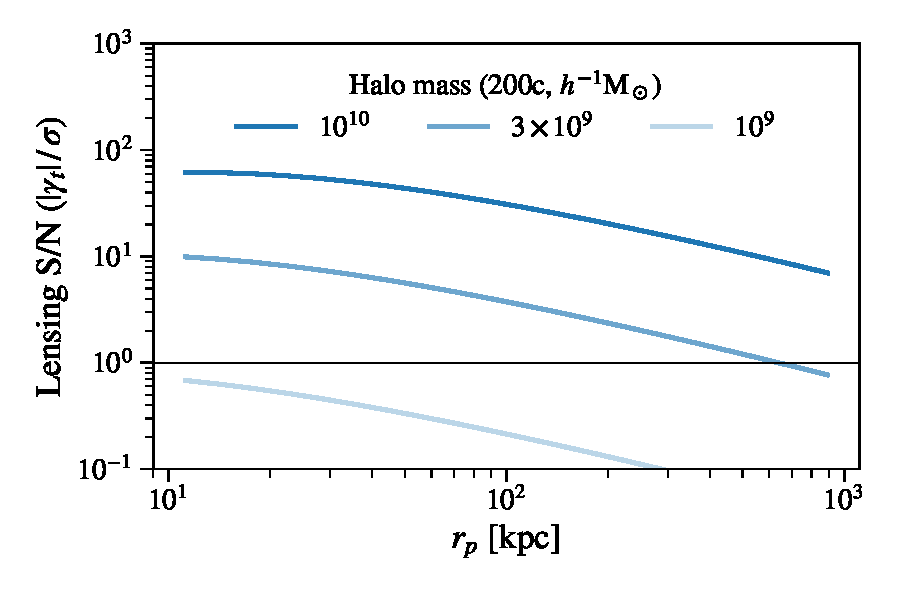
\includegraphics[width=\columnwidth]{halo_mass_lensing_sn}
\caption{
\label{fig:dwarf_sn} Lensing signal (reduced tangential shear; \textit{left}) and signal-to-noise (\textit{right}) for stacked samples of dwarf galaxies in three different mass bins (shown by different shapes of markers), each with width of 0.5 dex in mass. Two different density profiles are used for this calculation: the NFW profile (blue) and a NFW profile with a core (orange). 
The calculation assumes perfect selection of dwarf galaxies within the redshift range over which they are detectable by LSST. 
Source galaxies are assumed to be at $z=1.2$, with a surface number density of $50\,\amin^{-2}$, and a shear uncertainty of $\sigma_\gamma = 0.25$ per component.}
\end{figure}

We also calculate the shear signal for a modified NFW profile (with a core at the center; $\rho_\text{core}(r) = \rho_\text{NFW}(r) \times (1 -  e^{-3r/r_s})$) and show it in \figref{dwarf_sn}. We can see that the overall signal-to-noise does not change much with the profile. However, in order to distinguish the different profiles, we need to measure the shear at very small scales ($< 10$\,kpc). 



\ADW{We need to add a projection assuming a cored profile for the lenses. We need a concluding statement to bring this back to the dark matter questions raised in the intro. Should we include some discussion of PSF systematics?}
 % edit in dwarf-lensing.tex

\subsection{Galaxy Clusters \Contact{Susmita}}
\label{sec:halo_profile_clusters}
\Contributors{Susmita Adhikari, William A.\ Dawson, Nathan Golovich, David Wittman,  M.\ James Jee, Annika H.\ G.\ Peter, Daniel A.\ Polin, Robert Armstrong}

Galaxy clusters are the most massive gravitationally bound structures in the universe. The high matter density and high velocity dispersions of clusters make them ideal laboratories for testing dark matter self-interaction models in a very different regime from individual galaxies.
In the following section we discuss several probes that use galaxy clusters to constrain the nature of dark matter.  We show that current constraints from many different cluster-scale probes are of the order of $0.1$--$1\cmg$.  To understand why this is so, it is important to note that the average column density of a cluster-scale halo is of the order of $1 \g \cm^{-2}$.  Improved cross section constraints will come from a combination of the large statistical data sets that will be collected by LSST and other telescopes in the LSST era, and more sophisticated theoretical predictions for observables for specific SIDM models.

\vspace{1em} \noindent {\bf Distribution of matter and substructure}

As we describe below, the current best cluster-scale SIDM constraints come from the radial dark matter profiles of halos.  However, cluster-scale halos that consist of SIDM and CDM exhibit other differences, which may prove to be highly constraining given the vastly detailed LSST cluster data sets.  Significantly more theoretical work is required to project robust constraints in the LSST era for those probes.

\paragraph{Radial profile:} Interactions among dark matter particles allow for the exchange of energy between different parts of the halo. The high number of interactions near the dense central region of a dark matter halo increases the temperature, or the velocity dispersion, near the central region. This process can be thought of as a transfer of heat from the outer (hotter) parts of the halo to the inner (colder) region. The excess dispersion due to self interaction leads to flattening of the inner density of the halo, leading to the formation of a cored density profile. For cluster-scale halos, the high densities near the center make the timescales for thermalization shorter at a given cross section than they are for lower-mass objects (although it must be noted that low-mass halos are generally older and have a longer time to thermalize).  The short thermalization time is important because dark matter thus behaves as a fluid in the innermost part of cluster-scale halos, and can relax to a hydrostatic equilibrium configuration at the center of the halo, where baryons dominate the potential \citep{Kaplinghat:2015aga}.  Depending on the merger history, cluster-scale halos can be as cuspy as those in CDM-only simulations (for recent mergers), or relax to a hydrostatic equilibrium (for highly relaxed systems) in which the dark matter halo has a small but relatively dense core \citep{Robertson:2017mgj}.

Density profiles of massive galaxy clusters therefore serve as probes for SIDM. Clusters tend to be dark matter dominated outside the very central regions, and they are the only known systems where the matter distribution can be individually mapped to the virial radius using weak lensing. Strong lensing also provides a measure of cluster mass independent of the dynamical state. And stellar kinematics of the central galaxy can be used to measure the dark matter density profile in the innermost regions. LSST will produce an unrivaled catalog of strong and weak lensing measurement of cluster density profiles. This, in concert with X-ray mass estimates and stellar kinematics, will provide a strong test of the NFW dark matter density profile predicted by cold, collisionless dark matter \citep{Newman:2013,Kaplinghat:2015aga,Robertson:2018anx,Andrade:2019wzn}. Moreover, the strong lensing cross section is an additional probe of the density profile \citep{Robertson:2018anx}.  For hard-sphere scattering, cross section constraints are of the order of $0.1$--$1\cmg$, but without fully quantified systematic uncertainties.

\paragraph{Halo shape:} Apart from the density profile itself, in SIDM models, dark matter velocity distributions become more isotropic than in the CDM model, especially at the center of the halo.  Correspondingly,  the halo density profile becomes more spherical.  Historically, constraints from cluster and galaxy ellipticies \citep{Miralde-Escuda:2000} provided strong constraints on the cross section of SIDM; however, later investigations found these constraints to be somewhat optimistic \citep{Peter:2013}. 
Recent measurements of the shapes of cluster-scale dark matter halos include studies with: cluster members \citep{2018MNRAS.475.2421S},  X-rays \citep{Hashimoto:2007},  lensing \citep{Mandelbaum:2006, Evans:2009, Oguri:2010}, and combinations of observables \citep{Clampitt:2016, Sereno:2018}.  
Current constraints on the cross section are sensitive to the order of $\sigmam \sim 1 \cmg$.
Several groups have shown in $N$-body simulations that the effects of SIDM with a cross section of roughly $\text{(a few)}\times 0.1$--$1 \cmg$ are potentially observable, although baryons can alter the probability distribution function of halo shapes by an amount that is not yet robustly quantified \citep[\eg][]{Peter:2013, Robertson:2017mgj, Brinckmann:2018}.


\paragraph{Substructure:} Structures form hierarchically in the standard CDM scenario: small objects form first and merge to form larger mass structures such as galaxy clusters. These clusters continue to accrete smaller halos and some of these small structures survive as subhalos within the cluster. It is therefore interesting to study the distribution of substructures within larger halos, to understand how the distribution is affected by self interactions among dark matter particles. 

Subhalos can be affected by SIDM models in three different ways within a cluster. First, dark matter particles in subhalos can evaporate due to interactions with the particles in the host cluster. Subhalos lose mass when they enter a cluster. In the CDM scenario particles that are at larger radii and are loosely bound get stripped as the subhalo orbits within a cluster. In SIDM models, evaporation due to self-scattering leads to additional mass loss. Unlike tidal stripping, self-interactions can also affect the inner regions of the subhalos. Simulations show that evaporation is inefficient at increasing the subhalo disruption rate unless hard-sphere cross sections are of order $\sigmam \sim 10\cmg$, or subhalos are on nearly radial orbits through the cluster center \citep{2012MNRAS.423.3740V,Rocha:2012jg,Dooley:2016ajo}. 

While this generally means that the total subhalo mass function within the virial volume is largely unaffected relative to CDM, other effects of evaporation may be detectable. Measuring the mass and the profile around cluster satellites (especially as a function of orbit eccentricity) using galaxy--galaxy lensing to measure the mass-to-light ratio of subhalos can be a promising probe for dark matter physics \citep{Natarajan:2017sbo}. The lensing signal around subhalos is weak and will be contaminated by the cluster mass profile, so methods like subtracting the lensing signal from diametrically opposite points within the cluster can be used to extract the signal. Given the statistics of cluster galaxies in LSST, it is ideally suited for a study of the weak lensing signal of subhalos.  
Second, as subhalos are also tracers of the dark matter density field within the cluster, their orbits will be affected by the change in the potential of the cluster near the core relative to CDM.  This effect can lead to an imprint in the radial distribution of subhalos in clusters, generally by making the subhalos less concentrated toward the halo centers.

Third, non-expulsive interactions can lead to a drag force on subhalos.  This has several potentially interesting observable consequences.  The location of the splashback radius is sensitive to dynamics of subhalos within the cluster. The splashback radius is the boundary of the multistreaming region of a halo and is the largest apocenter of recently accreted objects \citep{Diemer:2014xya,Adhikari:2014lna}. The slope of the density profile of a halo falls off rapidly in a narrow localized region around this radius, and the splashback radius is observed as a minimum in the slope of the projected number density profile of galaxies \citep{More:2016vgs,Baxter:2017csy,Chang:2017hjt}.
The apocenter of the orbits of subhalos can change if there is extra drag beyond dynamical friction \citep{Kummer2018}.  
Therefore measuring the location of the splashback radius can help distinguish between different models of dark matter, although the difference between splashback locations in the CDM and SIDM scenarios has not yet been well quantified.

Similar to the situations discussed above and in merging clusters (Section~\ref{sec:merging_clusters}), the drag force due to non-expulsive interactions may also lead to offsets between the light distribution and dark matter distribution of individual satellites with respect to their subhalos. Small offsets between the subhalo and the galaxy within it may be detectable by indirect means: the potential gradient established by the dark matter at the position of the stellar centroid would induce a U-shaped warp in the stellar disk facing the direction of infall, and a longer-lasting disk thickening. Numerical simulations show these to be observable by current and next-generation photometric surveys under SIDM models with $0.5 \cmg \lesssim \sigmam \lesssim 1 \cmg$~\citep{Secco}. While S-shaped disks formed by tidal distortions of the stellar light profile are abundantly observed in cluster environments, indicating that they are readily induced by ``baryonic effects,'' these effects are not likely to generate prominent U-shaped warps. Such warps are only formed by a differential force on the disk and its halo, due to, for example, the SIDM drag.  The offset between a satellite galaxy and its subhalo may also be observed directly or statistically with strong lensing \citep{Massey2011,Massey:2017cwf}, but the magnitude of the effect is highly model-dependent (depending strongly on the angular and velocity dependence of the cross section).  Current limits are $\mathcal{O}(1\cmg)$ for specific non-hard-sphere models \citep{Harvey:2015hha}.  

\vspace{1em} \noindent {\bf Merging Galaxy Clusters \Contact{Nate?}}
\label{sec:merging_clusters}

% intro para
In the previous section, we considered subhalos to be minor merger events onto the main cluster.  Major cluster mergers can probe the nature of dark matter by serving as the biggest ``dark matter colliders'' on account of their high mass and large collision velocities. Dense halos falling together at thousands of km\,s$^{-1}$ provide an environment where the scattering of dark matter particles off each other would have observable effects.  The observable effects vary depending on the dark matter model and the configuration of the merger \citep{Kim:2016ujt}. 
Cluster mergers may also be able to distinguish between particle models that yield frequent scattering with low momentum transfer (as in a long-range force) and those that yield infrequent scattering with high momentum transfer (as with hard sphere or contact scattering) due to their differing phenomenology in the merger environment.  This is in contrast to the halo radial profile and shape constraints discussed in the previous section, for which the energy and momentum transfer rate matters most and for which there is no preferred direction in the problem.

% why LSST discovery is important
The best known example of a colliding cluster system is the Bullet Cluster, which has been frequently studied as a laboratory for SIDM \citep{Randall:2007ph,2017MNRAS.465..569R}. 
However, since a cluster merger is an eons-long process of which we have only a single snapshot, the measurement uncertainty is dominated by our very limited knowledge of the merger history. While it will remain critical to investigate individual clusters in great detail, the power of LSST lies in systematically analyzing a population of merging clusters with a consistent method, thereby constraining the properties of dark matter.
LSST will contribute to better and more robust constraints not only through the study of already known systems, but also by enabling the discovery of many more merging systems. Because mergers displace plasma from galaxies, they are best discovered by cross-correlation of LSST optically-detected clusters with radio and X-ray surveys \citep{Golovich:2018,Wilber2018}.

%offsets

The first SIDM constraints based on a merging galaxy cluster came from the Bullet Cluster, which was originally identified as an extremely hot X-ray cluster with two galaxy peaks. Higher resolution optical and X-ray imaging revealed a spectacular post-merger system with a clear X-ray cold front and shock. The spatial agreement of the galaxies and mass centroids obtained by weak lensing, and the disassociation of the intra-cluster medium (ICM) led to the constraint $\sigmam \lesssim 2 \cmg$ for hard-sphere scattering \citep{Markevitch2004,Randall:2007ph,2017MNRAS.465..569R,Robertson:2016qef}. Many other dissociative mergers have been found and studied, with roughly similar cross section limits \citep[but with greater systematic uncertainty, \eg][]{bradac2008}. 

After several ``dissociative'' mergers had been discovered, ensemble studies of the offsets between dark matter, galaxies, and gas were utilized to drive down the Poisson noise from inference on individual systems. \citet{Harvey:2015hha} modeled 72 subclusters within 30 merging systems to place the strongest constraint on SIDM ($\sigmam<0.47 \cmg$).
The study assumes a simplified drag force model where dark matter behaves similar to the ICM. However, \citet{Wittman:2017gxn} reanalyzed the sample including more comprehensive data. They identified several substantial errors that were driving the result and obtained a revised limit of $\sigmam \lesssim 2\cmg$.

The drag force model applies best to particle models with frequent interaction and low momentum transfer per interaction. In models with infrequent, high momentum transfer interactions (including hard-sphere scattering), dark matter particles may be scattered out of the cluster entirely. (Evaporation also occurs for small-angle scattering, though---see \citealt{Kahlhoefer:2013dca}.) This mass loss may be detected by comparing the mass-to-light ratio of merging clusters with those of non-merging clusters, on the assumption that the merger does not affect the galaxy light. This argument leads to a constraint of $\sigmam \lesssim 1 \cmg$, similar to current constraints on the drag model. However, the assumption that the galaxy light is unaffected is a source of uncertainty here. The LSST discovery of many more merging clusters, with six-band LSST photometry, will help us quantify this source of uncertainty. 

Several billion years post-pericenter, after a merging cluster has coalesced into a single cluster, SIDM will still create a cored dark matter distribution in the center of the cluster. For $\sigmam \sim 1 \cm^{2} \g^{-1}$, this core is $\roughly 100 \kpc$ (although the baryonic potential can alter the dark matter distribution). \citet{Kim:2016ujt} presented the effect of this on the brightest cluster galaxies (BCGs) up to 10 Gyr post-pericenter. They demonstrated a wobbling in the BCG as it is able to oscillate about the shallow potential for many oscillations. \citet{1703.07365} analyzed a small set of massive clusters and compared the BCG location with a strong lensing based estimate of the gravitational potential centroid. They compared these observations with hydro-CDM simulations to show that the observations suggest a cored dark matter halo in these clusters of $\roughly 10\kpc$. \citet{Harvey:2018uwf} recently studied cluster-scale halos in hydrodynamic simulations, and saw offsets that grew with cross section and halo mass, although with a smaller amplitude than the dark-matter-only simulations of \citet{Kim:2016ujt} implied. LSST will characterize thousands of relaxed clusters that invariably will have undergone a merger in their history. With deep and relatively high resolution imaging, LSST will allow for single snapshots of the BCG alignment in every massive cluster, and also for detection of faint strong lensing streaks in many of these systems.

% Esra added the text below
SIDM properties are sensitive to the separation between the centroid of the X-ray emitting hot plasma, i.e., intra-cluster medium (ICM), galaxies, and dark matter. Accurate measurements of the X-ray centroid of the X-ray emitting gas in clusters of galaxies requires sub-arcsec imaging with X-ray telescopes. The {\it Chandra} X-ray observatory with 0.5~arcsec FWHM PSF currently provides the most precise location of the ICM. Next-generation high spatial resolution X-ray observatories, \eg, {\textit Lynx} and {\textit AXIS} with much higher throughput, will provide accurate measurements of centers of high-redshift clusters ($z > 1$) in the 2030's and will enable tests of SIDM models over a much larger redshift range.
 % cluster people have organized subsubsections within clusters.tex

%\subsubsection{Halo Profiles of Bright Galaxies}
%\Contributors{Manoj?, Haibo?, Drew Newman?, Sean Tulin}
%\label{sec:halo_profile_galaxy}
% 
%\vspace{1em} \noindent {\bf Galaxy-Galaxy Lensing}
%\Contributors{?}
% 
%\vspace{1em} \noindent {\bf Caustics Structures}
%\Contributors{?}

